\documentclass[oneside,12pt]{amsart}
\usepackage[english]{babel}
\usepackage{graphicx}
\usepackage{float}
\usepackage{mathtools}
\usepackage{amsfonts}
\usepackage{amssymb}
\usepackage{siunitx}
\usepackage{amsthm}
\usepackage{enumitem}
\usepackage{stmaryrd}
\usepackage{multirow}
\usepackage[backend=bibtex,style=numeric]{biblatex}
\bibliography{Biblio}
\usepackage[a4paper, total={6in, 10in}]{geometry}
\graphicspath{{./}{}}% You can add the path for the images in the empty brackets 
\title{Study of Electrostatics: Generation and Measurement of Charge}
\author{Josh Goldfaden, Daniel Briseno}
\date{}
\newdimen\graph
\graph=4.2in
\newdimen\medgraph
\medgraph = 5.3in
\newdimen\smallgraph
\smallgraph = 3in
\newdimen\tinygraph
\tinygraph = 1.5in
\renewcommand{\arraystretch}{1.5}
\begin{document}
	\section{Abstract}
	In this series of experiments, Coulomb’s law was evaluated experimentally through first charging a top (T) strip of tape and a bottom (B) strip of tape and analyzing their interactions. In particular it was observed that (insert observations). Further, a virtual lab was conducted in which a hanging sphere was suspended, and its force body diagram was diagrammed and analyzed. Further, this sphere is placed in close proximity to a neighboring sphere attached to a rod, and their interactions were studied, specifically the magnitude of the Coulomb's force the suspended ball experienced was computed. It was found that (insert findings). One final virtual analysis that simulated the interaction between a suspended ball and the center of a charged rod. In this experiment, it was determined that (insert findings). In the final portion of the lab, Coulomb’s law was used to determine the discharge rate of a series of a virtual series of suspended spheres. 
	\section{Introduction}
	One experimental law of physics that is fundamental in understanding electrostatic forces is Coulomb’s law: 
	\begin{align}
		|\vec{F}^E_{12}| &= k_e \frac{|q_1 q_2|}{r_{12}^2}\\
		\vec{F}^E_{12} &= k_e \frac{|q_1 q_2|}{r_{12}^2} \hat{r}_{12} 
	\end{align}
	
	\indent This mathematical rule states that the magnitude of the force is the product of two charged particles, designated as $q_1$ and $q_2$ in units of Coulombs (unit of charge), and Coulomb’s constant (designated as $k_e$ with the unit N$\text{m}^2$/$\text{C}^2$) divided by the distance between the two particles squared, which is designated as $r_{12}$ with the unit $\text{m}^2$. It is noteworthy that Coulomb’s constant is a proportionality constant that relates different electric variables.\\ 
	
	\indent With respect to the implications of Coulomb’s law, in this particular lab, the electrostatic force exerted by a virtual charged sphere suspended by a rope  on a neighboring, virtual charged sphere attached to a rod. It is noteworthy that the sphere suspended by the rope is held at one 
	\section{Electric Field Due to a Line of Charge}
	\indent In this virtual lab, we wanted to measure the electrostatic force a charged rod exerts on a hanging test charge. (a hanging charged sphere). Recall from the introduction that we mathematically derived that the electric field due to a line of charge is:
	\begin{align*}
		|\vec{E}_{rod}| = \frac{kQ_{rod}}{r\sqrt{r^2+(L/2)^2}}
	\end{align*} 
	\indent Therefore, we would expect that empirically obtained values for the electric field exerted by a rod at different distances from a test charge would yield values which can be predicted by such a function.\\
	
	\indent In order to measure the electric field strength created by the rod at different radii, we hanged a ball with 35nC of charge and measured how much the ball was displaced when a charged rod of length 0.7104m was brought near it. Given the displacement of the ball and the ball's mass, we were able to determine the electric force acting on the ball. Given the charge of the ball, we were able to determine what the electric field magnitude due to the rod at the position of the ball. The results of our measurements are shown in Figure 1.\\
	
	\begin{figure}[h]
		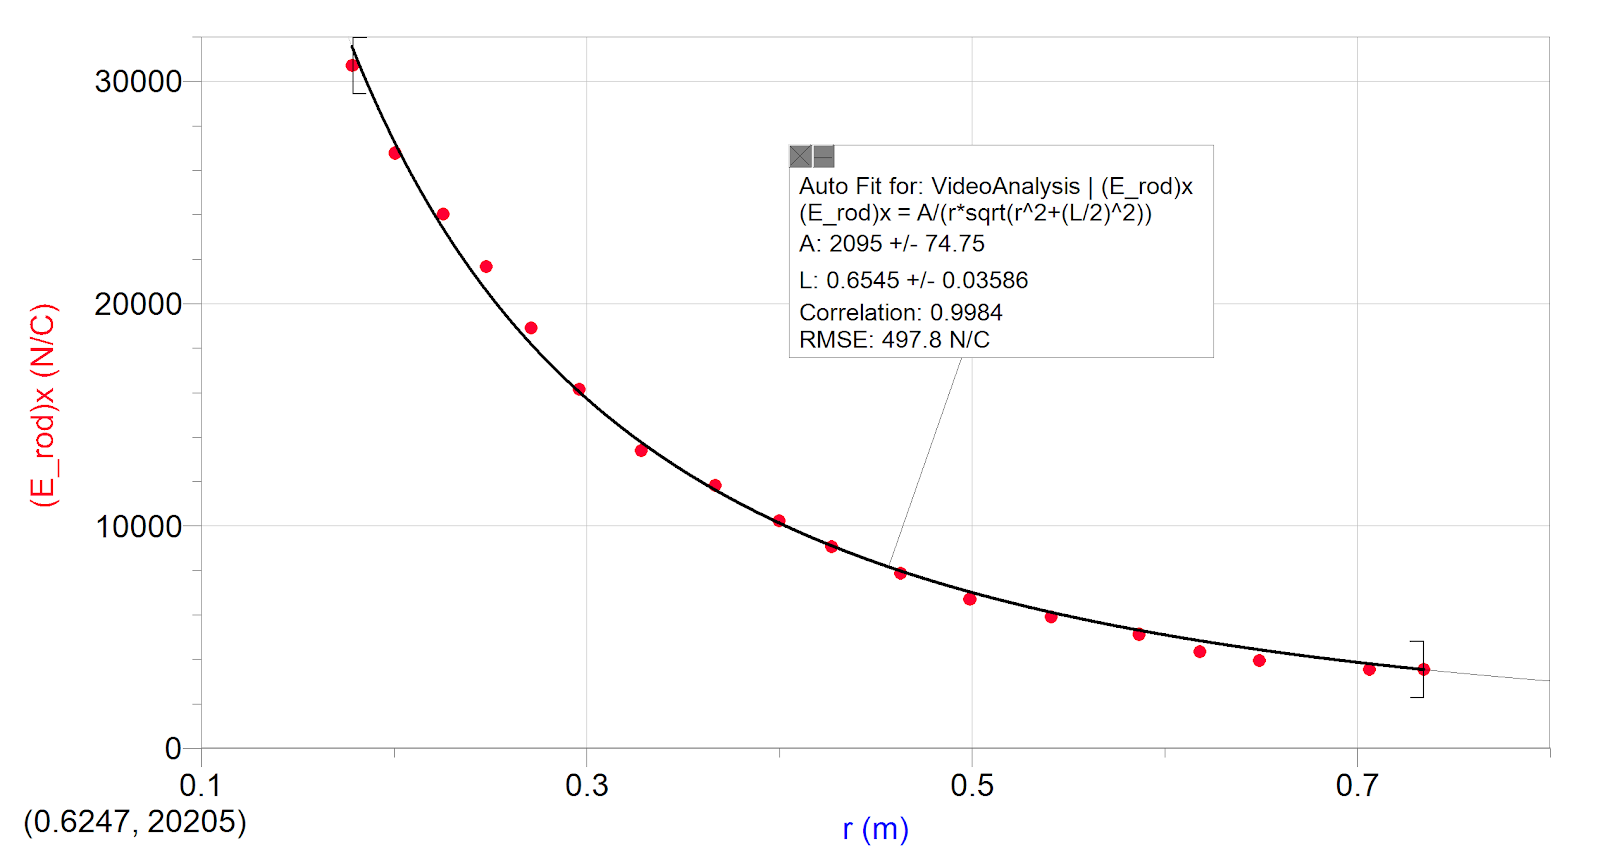
\includegraphics[width=\medgraph,scale=0.01]{FieldStrength.png}
		%h (here) - same location
		%t (top) - top of page
		%b (bottom) - bottom of page
		%p (page) - on an extra page5
		%! (override) - will force the specified location
		\caption{The electric field of the virtual rod (N/C) plotted against its distance from the charged sphere (m). 
		}
		\label{Fld}
	\end{figure}
	
	\indent Note that the line of best fit is in fact plotted by the theoretically obtained equation for the electric field magnitude created by a uniformly charged rod.\\
	
	\indent From this data we can also derive the charge present on the rod. Note that 
	\begin{align*}
	|\vec{E}_{rod}| = \frac{kQ_{rod}}{r\sqrt{r^2+(L/2)^2}} &= \frac{2095}{r^2+(L/2)^2} &&\text{From the best fit line}\\
	\implies 2095 &= kQ_{rod}\\
	\frac{2095}{k}&= Q_{rod}\\
	Q_{rod}&\approx 0.233\mu\text{C}
		\end{align*}
	
	
\end{document}